%%
% General report template.
%
\documentclass[12pt, a4paper, openany]{report}

% Packages for math, symbols, and formatting
\usepackage{amsmath, amssymb}
\usepackage{float} % Improved float handling
\usepackage{layout} % Show page layout
\usepackage{parskip} % Paragraph spacing
\usepackage{comment} % Commenting out large sections

% TikZ for figures
\usepackage{tikz}
\usetikzlibrary{calc, positioning, fit, arrows.meta, shapes}

\tikzset{
  transition/.style={font=\footnotesize, auto, inner sep=0.5ex},
  state/.style={font=\large, minimum size=1cm, draw, fill=white},
  statecolor/.style={state, draw=#1!70, fill=#1!30},
}

% Graphics and figures
\usepackage{graphicx}
\usepackage{wrapfig} % Text wrapping around figures
\usepackage{caption} % Customizing captions
\usepackage{subcaption} % Subfigures
\usepackage{rotating} % Rotating figures and tables

% Appendices
\usepackage[title,titletoc]{appendix}

% Bibliography and references
\usepackage[square,sort,comma,numbers]{natbib}

% Code listings
\usepackage{listings}
\usepackage{xcolor}
\definecolor{codegreen}{rgb}{0,0.6,0}
\definecolor{codegray}{rgb}{0.5,0.5,0.5}
\definecolor{codepurple}{rgb}{0.58,0,0.82}
\definecolor{backcolour}{rgb}{0.95,0.95,0.92}

\lstdefinestyle{mystyle}{
    backgroundcolor=\color{backcolour},
    commentstyle=\color{codegreen},
    keywordstyle=\color{magenta},
    numberstyle=\tiny\color{codegray},
    stringstyle=\color{codepurple},
    basicstyle=\ttfamily\footnotesize,
    breakatwhitespace=false,
    breaklines=true,
    captionpos=b,
    keepspaces=true,
    numbersep=5pt,
    showspaces=false,
    showstringspaces=false,
    showtabs=false,
    tabsize=2,
    otherkeywords={points} % Additional keywords
}
\lstset{style=mystyle}

% Page layout and geometry
\usepackage[top=20mm, bottom=20mm, left=20mm, right=30mm]{geometry}

% Typographical adjustments
\usepackage[expansion=false]{microtype}

% Ensuring figures appear after their first mention
\usepackage{flafter}
% Customizing chapter headings
\usepackage{titlesec}
\titleformat{\chapter}[display]{\huge\bfseries}{\chaptertitlename~\thechapter}{0.5cm}{\bfseries}
\titlespacing{\chapter}{0pt}{-1cm}{1cm}

% Header and footer configuration
\usepackage{fancyhdr}
\pagestyle{fancy}
\fancyhf{}
\fancyfoot[C]{\thepage} % Page number in the center of the footer
\renewcommand{\headrulewidth}{0pt} % Remove header line
\renewcommand{\footrulewidth}{0pt} % Remove footer line

% Line spacing adjustment
\usepackage{setspace}
\setstretch{0.9}

% Table handling
\usepackage{array}
\floatstyle{plaintop}
\restylefloat{table}

% Numbering equations by section
\numberwithin{equation}{section}

% Acronyms
\usepackage{acronym}

% Font encoding
\usepackage[T1]{fontenc}

% Improved table of contents and references
\usepackage[colorlinks=true, allcolors=blue]{hyperref}

\usepackage{maori}

%%
% Commands
%
\newcommand{\HRule}{\rule{\linewidth}{0.5mm}}
\renewcommand{\bibname}{References}
% \usepackage{biblatex}
% \addbibresource{url.bib}

%%
%	Document Starts Here
% 	Initial Sections
%
\begin{document}
\begin{titlepage}
\begin{center}

{ \large
	Water 1      \\
	Infrastructure Discipline \\
	TONKIN \& TAYLOR 
} \\[3cm]

{ \huge \bfseries 
	Variational Autoencoder for Climate Change-Driven Hydrological Stochastic Data Generation
} \\[0.5cm]

\HRule \\[3cm]

{ \large
	Martin Wright						
} \\[3cm]
{ 
	\emph{Supervisors:}					\\
	Sam Reed						\\
    Amy Waters                  \\
	David Leong					\\[3cm]
	October 2025
}


\end{center}
\end{titlepage}
\thispagestyle{empty} % Keep the title page without numbering
\setcounter{page}{1}
\pagenumbering{roman}

\newpage
\section*{Acknowledgements}
I would like to acknowledge ...
\section*{Declaration}
I declare that this report and all in it has been written independantly by myself.

\textbf{Martin Wright, October 2025}
% Remove \thispagestyle{plain} to keep fancy page numbering

\newpage
\tableofcontents
\listoffigures
\listoftables

%	Main Sections
%
\newpage
\setcounter{page}{1}
\pagenumbering{arabic}

\chapter{Introduction} \label{Section:Intro}

Global Climate Models (GCMs) provide the primary basis for understanding future climate under 
alternative emissions scenarios, yet their coarse spatial resolution 
limits direct application for regional impact assessments. Downscaling techniques 
bridge this gap by translating GCM outputs to the finer scales required by local 
decision-making processes. For Auckland's metropolitan water supply system, this 
is critical for long-term planning. 

Watercare operates the Integrated Source Management Model (ISMM) 
to optimise conjunctive use of their water reservoirs, groundwater sources, and rivers. The 
ISMM program requires long daily sequences of rainfall and potential 
evapotranspiration (PET) to evaluate system yields under current and future climate conditions.

Previous work for Watercare developed a methodology combining dynamically downscaled GCM 
projections with stochastic weather generation. Historical rainfall records were perturbed 
using shifts in gamma distribution parameters derived from downscaled projections, then 
extended using the Stochastic Climate Library (SCL) to produce 1000-year datasets. 
This approach has enabled assessment of water supply resilience under Representative 
Concentration Pathways 4.5 and 8.5 for mid-century (2040) and late-century (2090) time 
horizons, providing valuable insights for infrastructure planning.

However, several limitations constrain the robustness of this framework for future assessments. 
Perturbation methods based on fitted parametric distributions struggle to represent extreme 
rainfall events that are rare in historical records but critical for water supply security. 
Stochastic weather generators reproduce statistical variability from training data rather than 
generating physically plausible extremes beyond observed ranges. Traditional generators also 
treat daily weather as conditionally independent given the previous day, failing to capture 
the full temporal coherence of multi-day storm systems and drought evolution. Furthermore, 
the existing framework incorporates PET as simplified annually repeating functions, weakening 
representation of compound climate stressors such as concurrent drought and high evaporative 
demand.

Recent advances in deep generative models offer alternative approaches that may address these 
limitations. Variational Autoencoders (VAEs) learn flexible representations of complex data 
distributions without assuming parametric forms, and their structured latent spaces enable 
controlled generation of samples with varying characteristics. This research extends the VAE 
framework by incorporating learned latent dynamics to capture temporal evolution of weather 
patterns. Unlike standard VAEs that treat each observation independently, sequential VAEs learn 
how latent representations evolve from one day to the next, enabling generation of temporally 
coherent multi-day sequences.

The model is trained on bias-corrected, dynamically downscaled GCM projections for both 
historical and future scenarios, learning spatial weather patterns, their temporal evolution, 
and how these characteristics shift under climate change. By combining strategic latent space 
sampling with learned dynamics and temporal conditioning, the approach aims to generate 
thousand-year synthetic datasets suitable for ISMM while addressing key limitations of existing 
methods. The research develops a sequential VAE architecture for multi-variable spatial weather 
fields, implements recurrent latent dynamics using Gated Recurrent Units, and demonstrates 
controlled generation of extreme scenarios through latent space sampling. The ultimate 
objective is to provide Watercare with enhanced capability for assessing water supply 
resilience under climate change, particularly for extreme events that pose greatest risk to 
system reliability yet remain poorly represented in traditional synthetic weather datasets.

\chapter{Background}

\section{Auckland's Water Supply System and ISMM}

Auckland's metropolitan water supply serves over 1.7 million people across New Zealand's 
largest urban area. The system comprises multiple sources managed conjunctively: surface water 
reservoirs in the Hunua and Waitakere Ranges, groundwater from various aquifer systems, and 
river abstractions from the Waikato River. This diversity provides resilience against 
individual source failures but requires sophisticated operational management to balance 
competing demands, environmental constraints, and storage dynamics across the integrated system.

The Integrated Source Management Model (ISMM) is Watercare's primary decision-support tool 
for 
long-term planning and operational optimisation. The model simulates daily water movements 
through the entire supply system, tracking reservoir storage levels, aquifer drawdown, river 
flows, and treatment plant capacities. Environmental flow requirements, infrastructure 
constraints, and operational rules govern how water can be extracted and transferred between 
sources. To evaluate system performance---particularly the reliable yield, defined as the 
maximum demand that can be met with acceptable security of supply---the ISMM requires input 
sequences spanning centuries. This length is necessary to adequately sample low-frequency 
variability in rainfall and to estimate the probability of severe multi-year droughts that 
could challenge system resilience.

Previous climate change impact assessments for Watercare relied on producing these extended 
sequences through a two-stage process. Dynamically downscaled GCM projections provided daily 
rainfall and temperature data at approximately 5\,km resolution across the supply catchments. 
These projections were bias-corrected against observed records to improve agreement with 
historical statistics. Monthly gamma distributions were then fitted to both historical and 
projected rainfall series, and the shifts in distribution parameters between time periods 
were applied to perturb the observed historical record. This perturbation preserved the 
day-to-day temporal structure of observed weather while embedding projected changes in rainfall 
statistics. The perturbed records were then extended using the Stochastic Climate Library, 
which generated multiple stochastic replicates that were concatenated to produce sequences 
exceeding one thousand years. This methodology provided workable datasets for ISMM and yielded 
insights into system vulnerability under RCP4.5 and RCP8.5 scenarios.

\section{Limitations of Current Methodology}

The perturbation-based approach assumes that future rainfall can be adequately represented by 
shifting the parameters of distributions fitted to historical data. For bulk statistics such as 
monthly means and standard deviations, this assumption is reasonable and well-supported by theory. 
However, extreme events occupy the tails of rainfall distributions where sample sizes are 
inherently small. Fitting parametric distributions to limited extreme samples and then 
extrapolating through parameter shifts introduces substantial uncertainty. The gamma 
distribution, while flexible, may not accurately represent the tail behaviour of precipitation, 
particularly for sub-daily or multi-day accumulations where extreme value theory suggests 
alternative distributions may be more appropriate.

Further, one of the arguments for the augmented delta-shift method was that GCMs couldn't model ``unknown 
unknowns'' \cite{tnt}. However, this is not actually true; for example, volcanic forcings (one of
the examples explicitly given) \textit{are} actually modelled during the historical calibration
run.

The SCL faces a practical constraint regarding multivariate generation: it can either maintain 
spatial co-variance across sites for a single variable, or temporal co-variance between 
multiple variables at a site, but not both simultaneously within its current framework. For the 
Watercare application, accurate spatial co-variance of rainfall across the supply catchments 
was deemed more critical than dynamic coupling between rainfall and PET. Consequently, PET was 
incorporated as monthly averaged values that repeat annually, scaled according to future 
projections but lacking day-to-day variability. This simplification weakens the ability to 
model compound events where anomalously high temperatures and evaporative demand coincide with 
rainfall deficits, amplifying drought stress. Such compound events are particularly concerning 
under climate change, where rising temperatures are projected to increase atmospheric water 
demand even as precipitation patterns shift.

\section{Challenges with Bias Correction}

Bias correction has become standard practice in climate impact modelling, with quantile 
mapping (QM) and its variants widely adopted across sectors. These methods align GCM output 
distributions with observed distributions by constructing transfer functions that map modelled 
quantiles to observed quantiles. When applied to future projections, the method assumes that 
the biases present in historical simulations persist into the future, allowing the same 
transfer functions to correct future data. This assumption of bias stationarity is convenient 
but physically questionable, as the sources of GCM biases, such as insufficient resolution of 
orographic precipitation or imperfect representation of convective processes may change as 
the climate state changes.

Chandel et al.~\cite{Chandel_2024} demonstrated that aggressive bias 
correction can distort or suppress the climate change signals that GCMs are designed to project. 
Their analysis showed that quantile-mapped GCM fields can become statistically 
indistinguishable from quantile-mapped random fields, suggesting that the correction process 
forces GCM outputs to conform so closely to historical observations that future climate signals 
are obscured. The climate change signal in a GCM projection emerges from the model's 
representation of radiative forcing, circulation changes, and thermodynamic responses. When 
quantile mapping forces future distributions to align with historically observed distributions, 
it may inadvertently remove physically meaningful changes in variability, extreme event 
frequency, or relationships between variables.

This tension between improving historical fidelity and preserving future climate signals 
represents a fundamental challenge for impact modelling. Uncorrected GCM outputs often contain 
substantial biases that render them unsuitable for direct use in impact models calibrated to 
historical conditions. Yet aggressive correction risks undermining the very climate change 
information the GCMs provide. The optimal approach likely lies in methods that improve GCM 
outputs without completely subordinating them to historical statistics, preserving the physical 
relationships and change signals while reducing systematic biases.

\chapter{Literature Review}

\section{Climate Model Downscaling and Bias Correction}

Global Climate Models simulate Earth's climate system by solving fundamental equations 
governing atmospheric dynamics, radiative transfer, and energy balance on discretized grids. 
The computational cost of these simulations constrains spatial resolution, with most CMIP6 
models operating at 100--200\,km grid spacing. At these resolutions, regional climate features 
influenced by topography, land-sea contrasts, and mesoscale circulation patterns cannot be 
resolved. New Zealand's complex topography, with mountain ranges that generate substantial 
orographic precipitation enhancement, exemplifies the challenge: a single GCM grid cell may 
encompass coastal lowlands, mountain peaks, and lee-side rain shadows that experience vastly 
different local climates.

Dynamical downscaling addresses this limitation by nesting regional climate models (RCMs) 
within GCM simulations. The RCM uses the GCM output as boundary conditions but solves 
atmospheric equations at much finer resolution, typically 5--50\,km grid spacing. This allows 
explicit representation of topographic effects and regional circulation features. For New 
Zealand, NIWA has developed a suite of dynamically downscaled projections using the Conformal 
Cubic Atmospheric Model (CCAM) at 5\,km resolution, driven by selected CMIP6 GCMs. These 
projections provide daily precipitation, temperature, and radiation fields suitable for 
hydrological applications.

However, dynamical downscaling does not eliminate model biases. RCMs inherit boundary condition 
biases from driving GCMs and introduce their own biases through imperfect parameterisations of 
sub-grid processes. Consequently, bias correction is typically applied before using downscaled 
projections in impact models. Quantile mapping has emerged as the dominant approach, 
constructing transfer functions that align modelled quantiles with observed quantiles from a 
reference dataset. The method adjusts not just the mean but the entire distribution, improving 
representation of variability and extremes.

Despite its widespread adoption, quantile mapping faces theoretical and practical challenges. 
The assumption of bias stationarity---that biases present in the historical period persist 
unchanged into the future---lacks physical justification. Climate change may alter the nature 
and magnitude of model biases as the climate state evolves. More fundamentally, Chandel et 
al.~\cite{Chandel_2024} demonstrated that quantile mapping can suppress or distort the climate 
change signals in GCM projections. Their analysis compared quantile-mapped GCM outputs with 
quantile-mapped random fields and found minimal statistical distinction, suggesting the 
correction process forces future projections to resemble observations so closely that 
physically meaningful climate changes are obscured.

This finding challenges a foundational assumption in climate impact modelling: that 
bias-corrected GCM projections provide reliable information about future climate changes. If 
the correction process distorts change signals, then impact assessments based on corrected data 
may misrepresent future risks. The implications are particularly concerning for extreme events, 
where the magnitude of projected changes often exceeds the magnitude of historical biases, 
making the separation of bias from signal especially difficult.

\section{Stochastic Weather Generators}

Stochastic weather generators produce synthetic weather sequences by modelling the statistical 
properties of observed data. Early generators focused on precipitation occurrence and amount, 
using Markov chains to represent wet/dry day sequences and parametric distributions for 
rainfall amounts on wet days. More sophisticated generators incorporate multiple variables with 
inter-variable correlations, spatial dependence across sites, and consistency with observed 
statistical properties across multiple timescales.

The Stochastic Climate Library used in previous Watercare assessments represents an advanced 
implementation that preserves spatial correlation across sites through careful calibration of 
multivariate distributions. The generator conditions on specified marginal distributions and 
correlation structures, allowing for the production of synthetic sequences that match desired 
statistical properties while extending beyond the length of observed records. This capability 
is essential for water resources applications requiring multi-century sequences to estimate 
low-probability supply failures.

However, weather generators face an inherent limitation: they reproduce the statistical 
envelope of their conditioning data but do not extrapolate beyond it. The generator resamples 
and recombines patterns present in observations, maintaining statistical consistency but not 
exploring genuinely novel conditions. For climate change applications, this means the generator 
can produce sequences matching perturbed statistics derived from climate projections, but it 
cannot generate extreme events substantially beyond those used for calibration. The range of 
generated variability is bounded by the calibration dataset.

Recent developments in weather generator methodology have explored various approaches to 
address this limitation. Some methods explicitly model extreme value distributions separately 
from bulk distributions, using generalised extreme value or generalised Pareto distributions 
for tail behaviour. Others incorporate non-stationary models where distribution parameters vary 
over time according to climate indices or trends. Multi-site generators that preserve spatial 
correlation patterns provide improved representation of regional-scale events. Despite these 
advances, the fundamental challenge remains: extrapolating beyond observed variability requires 
assumptions about how statistical properties change, and these assumptions introduce 
uncertainty.

\section{Machine Learning for Weather and Climate}

The application of machine learning to weather and climate problems has expanded rapidly, 
driven by increasing computational power, availability of large datasets, and algorithmic 
innovations. Early applications focused on pattern recognition and classification tasks such 
as identifying weather regimes or detecting extreme events in climate model output. More 
recently, generative models have been applied to weather prediction, downscaling, and synthetic 
data generation.

Variational Autoencoders have emerged as a powerful framework for learning complex probability 
distributions and generating samples from high-dimensional data. VAEs explicitly model data 
distributions through a probabilistic encoder-decoder structure, providing both training 
stability and a structured latent space that enables controlled generation. The regularization 
of latent space to a known distribution creates natural mechanisms for sampling and 
interpolation. Oliveira et al.~\cite{vae-synthesis} demonstrated VAE application to 
precipitation field generation, showing that latent space sampling could control scenario 
extremity. Their approach trained a VAE on monsoon precipitation data, then generated extreme 
scenarios by sampling from the distribution tails. 
Quantile-quantile plots validated that samples from low-probability latent regions produced 
precipitation fields with characteristics matching observed extreme events. This established 
the principle that VAE latent space structure enables controlled generation of extremes without 
requiring explicit conditioning variables or separate extreme value models.

The standard VAE framework treats each observation independently, which is suitable for 
generating spatial fields but cannot capture temporal dependencies essential for multi-day 
weather sequences. This limitation motivates extension to sequential VAEs that incorporate 
learned temporal dynamics, enabling generation of coherent time series rather than independent 
snapshots. For climate applications, machine learning approaches offer both opportunities and 
challenges. The ability to learn complex non-linear relationships directly from data without 
restrictive parametric assumptions is attractive, particularly for representing multivariate 
dependencies and spatial patterns. However, machine learning models generally require large 
training datasets, may struggle to extrapolate beyond training data ranges, and provide less 
transparent representations than traditional statistical models. Validation and interpretation 
require careful attention to ensure generated data possess appropriate physical constraints 
and statistical properties.

\section{Temporal Dynamics}

Modelling temporal sequences requires capturing dependencies across time. Recurrent neural 
networks provide a natural framework for 
sequential modelling through hidden states that carry information forward through time. The 
hidden state at each timestep is updated based on the current input and previous hidden state, 
enabling the network to maintain memory of past observations. Gated Recurrent Units (GRU) 
address the vanishing gradient problem that limits standard RNNs' ability to 
capture long-range dependencies. The GRU architecture uses reset and update gates to control 
information flow, allowing the network to learn which aspects of past states to retain and 
which to discard \cite{GRU}. This gating mechanism proves particularly effective for weather sequences 
where some features (like large-scale circulation patterns) evolve slowly while others (like 
local precipitation) change rapidly.

In the context of sequential VAEs, GRU networks model latent dynamics through a transition 
function that predicts the distribution of latent codes at time $t$ given the latent code at 
time $t-1$ and the recurrent hidden state. This architecture captures temporal dependencies at 
two levels: the latent codes themselves evolve over time, and the hidden state maintains 
additional memory of the sequence history. The dual representation allows the model to capture 
both fast timescale dynamics (day-to-day changes in weather) and slower processes (gradual 
evolution of seasonal conditions or multi-week circulation patterns).

Training sequential generative models faces the challenge of exposure bias. During training 
with teacher forcing, the model receives ground-truth observations at each timestep, allowing 
it to correct for any errors made at previous steps. During generation, the model must rely on 
its own predictions, and errors can accumulate over long sequences. Various approaches address 
this problem, including scheduled sampling (gradually reducing teacher forcing during training), 
professor forcing (using adversarial training to match training and generation conditions), 
and rollout-based objectives that explicitly train on self-generated sequences.

For weather sequence generation, capturing appropriate timescales of variability is critical. 
Daily weather exhibits persistence due to the movement of synoptic systems with characteristic 
timescales of days. Seasonal cycles operate at annual timescales. Interannual variability from 
climate modes like the El Niño-Southern Oscillation introduces dependencies spanning years. A 
successful sequential model must balance these multiple timescales, maintaining short-term 
coherence while allowing longer-term variability. The latent dynamics architecture provides 
flexibility to learn these multi-scale dependencies from data rather than imposing them through 
model structure.

\section{Generative AI}

The term ``generative AI'' has become widly popularised as a way to refer to state-of-the art 
foundational models such as stable diffusion or SoRA. However, the term itself has a meaning
more grounded in the idea of a model being able to generate reasonable outputs without the
need for complex input. This differs greatly to traditional applications of neural networks
prior, where a network of perceptrons learn the optimum weights \& biases to transform a 
complex, high-dimensional input into an output. Put simply, $f: x \rightarrow y$.

\subsection{Variational Autoencoders}

The traditional autoencoder is made up of the encoder and decoder, where the decoder output 
shape matches that of the input into the encoder. The encoder takes the input $x$ and 'reduces'
it down into some value $z$, which represents some point in a $d$ dimensional abstact space
refered to as ``latent'' space.

Much noise has been made lately about researching the application of generative adversarial
networks (GANs) and stable diffusion models for gridded weather synthesis, due to their 
successes in the image generation space. The issue with this thinking, however, is that 
weather synthesis is done on a much coarser grid and for discretely different purposes.
While the outputs may experience fuzzing, this smoothness is representative of the inherit
variance in weather patterns, and smooths out over long simulations. Perfect for simulating
climate change impacts over long time frames.

The variational autoencoder utilises stochastics to improve the performance of an 
autoencoder by enriching this latent space into a prior and posterior distribution, forcing
it to its Gaussian representation \cite{vae}.

\subsubsection{$\beta$-VAE}

While the VAE achieves limited disentangling performance, it does not scale to more complex
datasets such as image generation. The $\beta$-VAE is a deep unsupervised approach which
augments the standard VAE with the $\beta$ hyperparameter that modulates the learning 
constraints being applied to the model \cite{beta-vae}. The case $\beta=1$ matches the 
performance of the VAE, but for cases $\beta>1$, the model learns a more efficient latent 
representation of the input data. 

\chapter{Scope} \label{Section:Scope}

\newpage
\chapter{Methods}

This study develops a hybrid Variational Autoencoder–Generative Adversarial Network (VAE-GAN) framework for generating synthetic rainfall and potential evapotranspiration (PET) sequences for use in Watercare’s Integrated Source Management Model (ISMM). The framework integrates information from two sources: (i) historical observations and reanalysis datasets, which provide the empirical basis for learning spatial–temporal weather patterns, and (ii) climate projections from downscaled Global Climate Models (GCMs), which provide the climate change signals that must be preserved in the synthetic sequences.

The methodology consists of three stages. First, a VAE is trained using historical fields to learn a structured probabilistic latent space representation of rainfall and PET. Second, GCM-derived perturbations are mapped into the latent space through bias correction and delta-shift methods. Third, a VAE-GAN decoder is employed to generate synthetic weather fields that reflect both the historical climatology and projected climate signals, while the adversarial discriminator improves realism and fidelity, particularly at the extremes.

\section{Data}


The downscaled GCM data was provided by the ministry for the environment \cite{GCM} 
\cite{user-guidance}. From the CMIP 6 ensemble, six models were chosen and dynamically
downscaled. These mpdels were chosen based on their performance over the historical 
baseline and assessed using specific, technical performance. Here, Gibson et al.
\cite{GCM} look at process-based metrics, model independence and spread in equilibrium
climate sensitivity.

\subsection{Dynamic Downscaling} \label{Section:DynamicDownscaling}

The models were downscaled with the Conformal Cubic Atmospheric Model (CCAM) \cite{CCAM}.
This method uses a "variable-resolution conformal-cubic grid" to recreate a finer resolution 
over the region of interest alognside a, relatively, high resolution (12-35km) grid over the
wider pacific area.

The first three of the chosen six models (ACCESS-CM2, EC-Earth3, NorESM2-MM) used CCAM through
spectral nudging \cite{user-guidance}; in other words, the regional climate model (RCM) is 
biased towards the GCM data by only "nudging" the long wavelengths/large-scale features of 
the RCM's simulated fields to those of the GCM. Here, the RCM is biased towards the atmospheric
fields, sea surface temperatures and sea ice concentrations of the GCM.

The three other models (AWI-CM-1-1-MR, CNRM-CM6-1, GFDL-ESM4) were simulated using free-
running atmospheric calculations but with sea surface temperature and sea ice concentrations   
being provided externall by the larger GCM.

\subsection{Downscaled GCM's}

The `\textit{National climate projections for Aotearoa New Zealand}' project produced
dynamically downscaled climate projections, as descibed above in subsection \ref{Section:DynamicDownscaling}.


\section{Model Architecture}

Oliveira et al. \cite{vae-synthesis} included temporal modelling directly into the VAE model. 
What we are proposing here, is instead to use GRU to model the temporal dependencies, $p(z_t|
z_{t-1})$.

\newpage
\chapter{Results}

\section{Statistics}

From the distribution comparison and quantile-quantile (Q-Q) plot in figure 
\ref{fig:statistics}

\begin{figure}[h!]
    \centering
    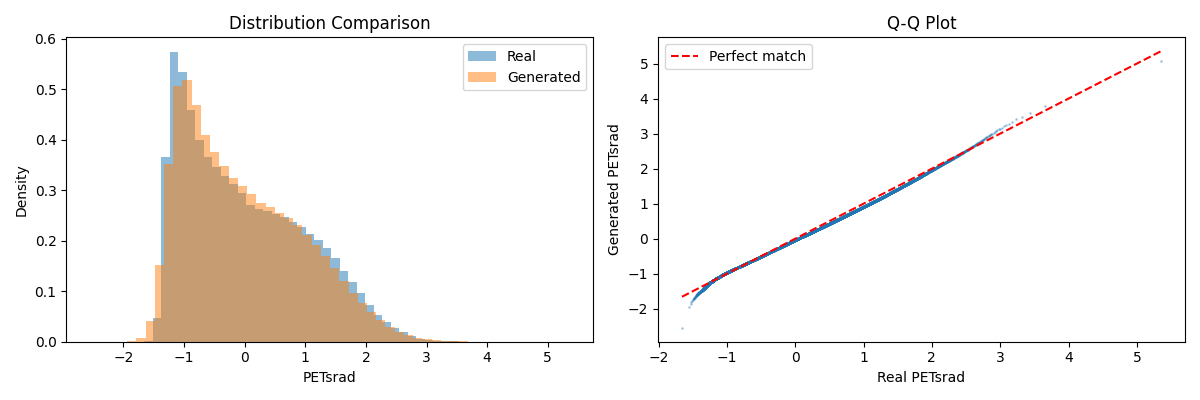
\includegraphics[scale=0.5]{figures/Stats.png}
    \caption{Statistical comparison of model training \& output data}
    \label{fig:statistics}
\end{figure}

\section{Model Outputs}

Taking random samples from the historical database and recreating their latent 
space representations, the following results are produced.

\begin{figure}[h!]
    \centering
    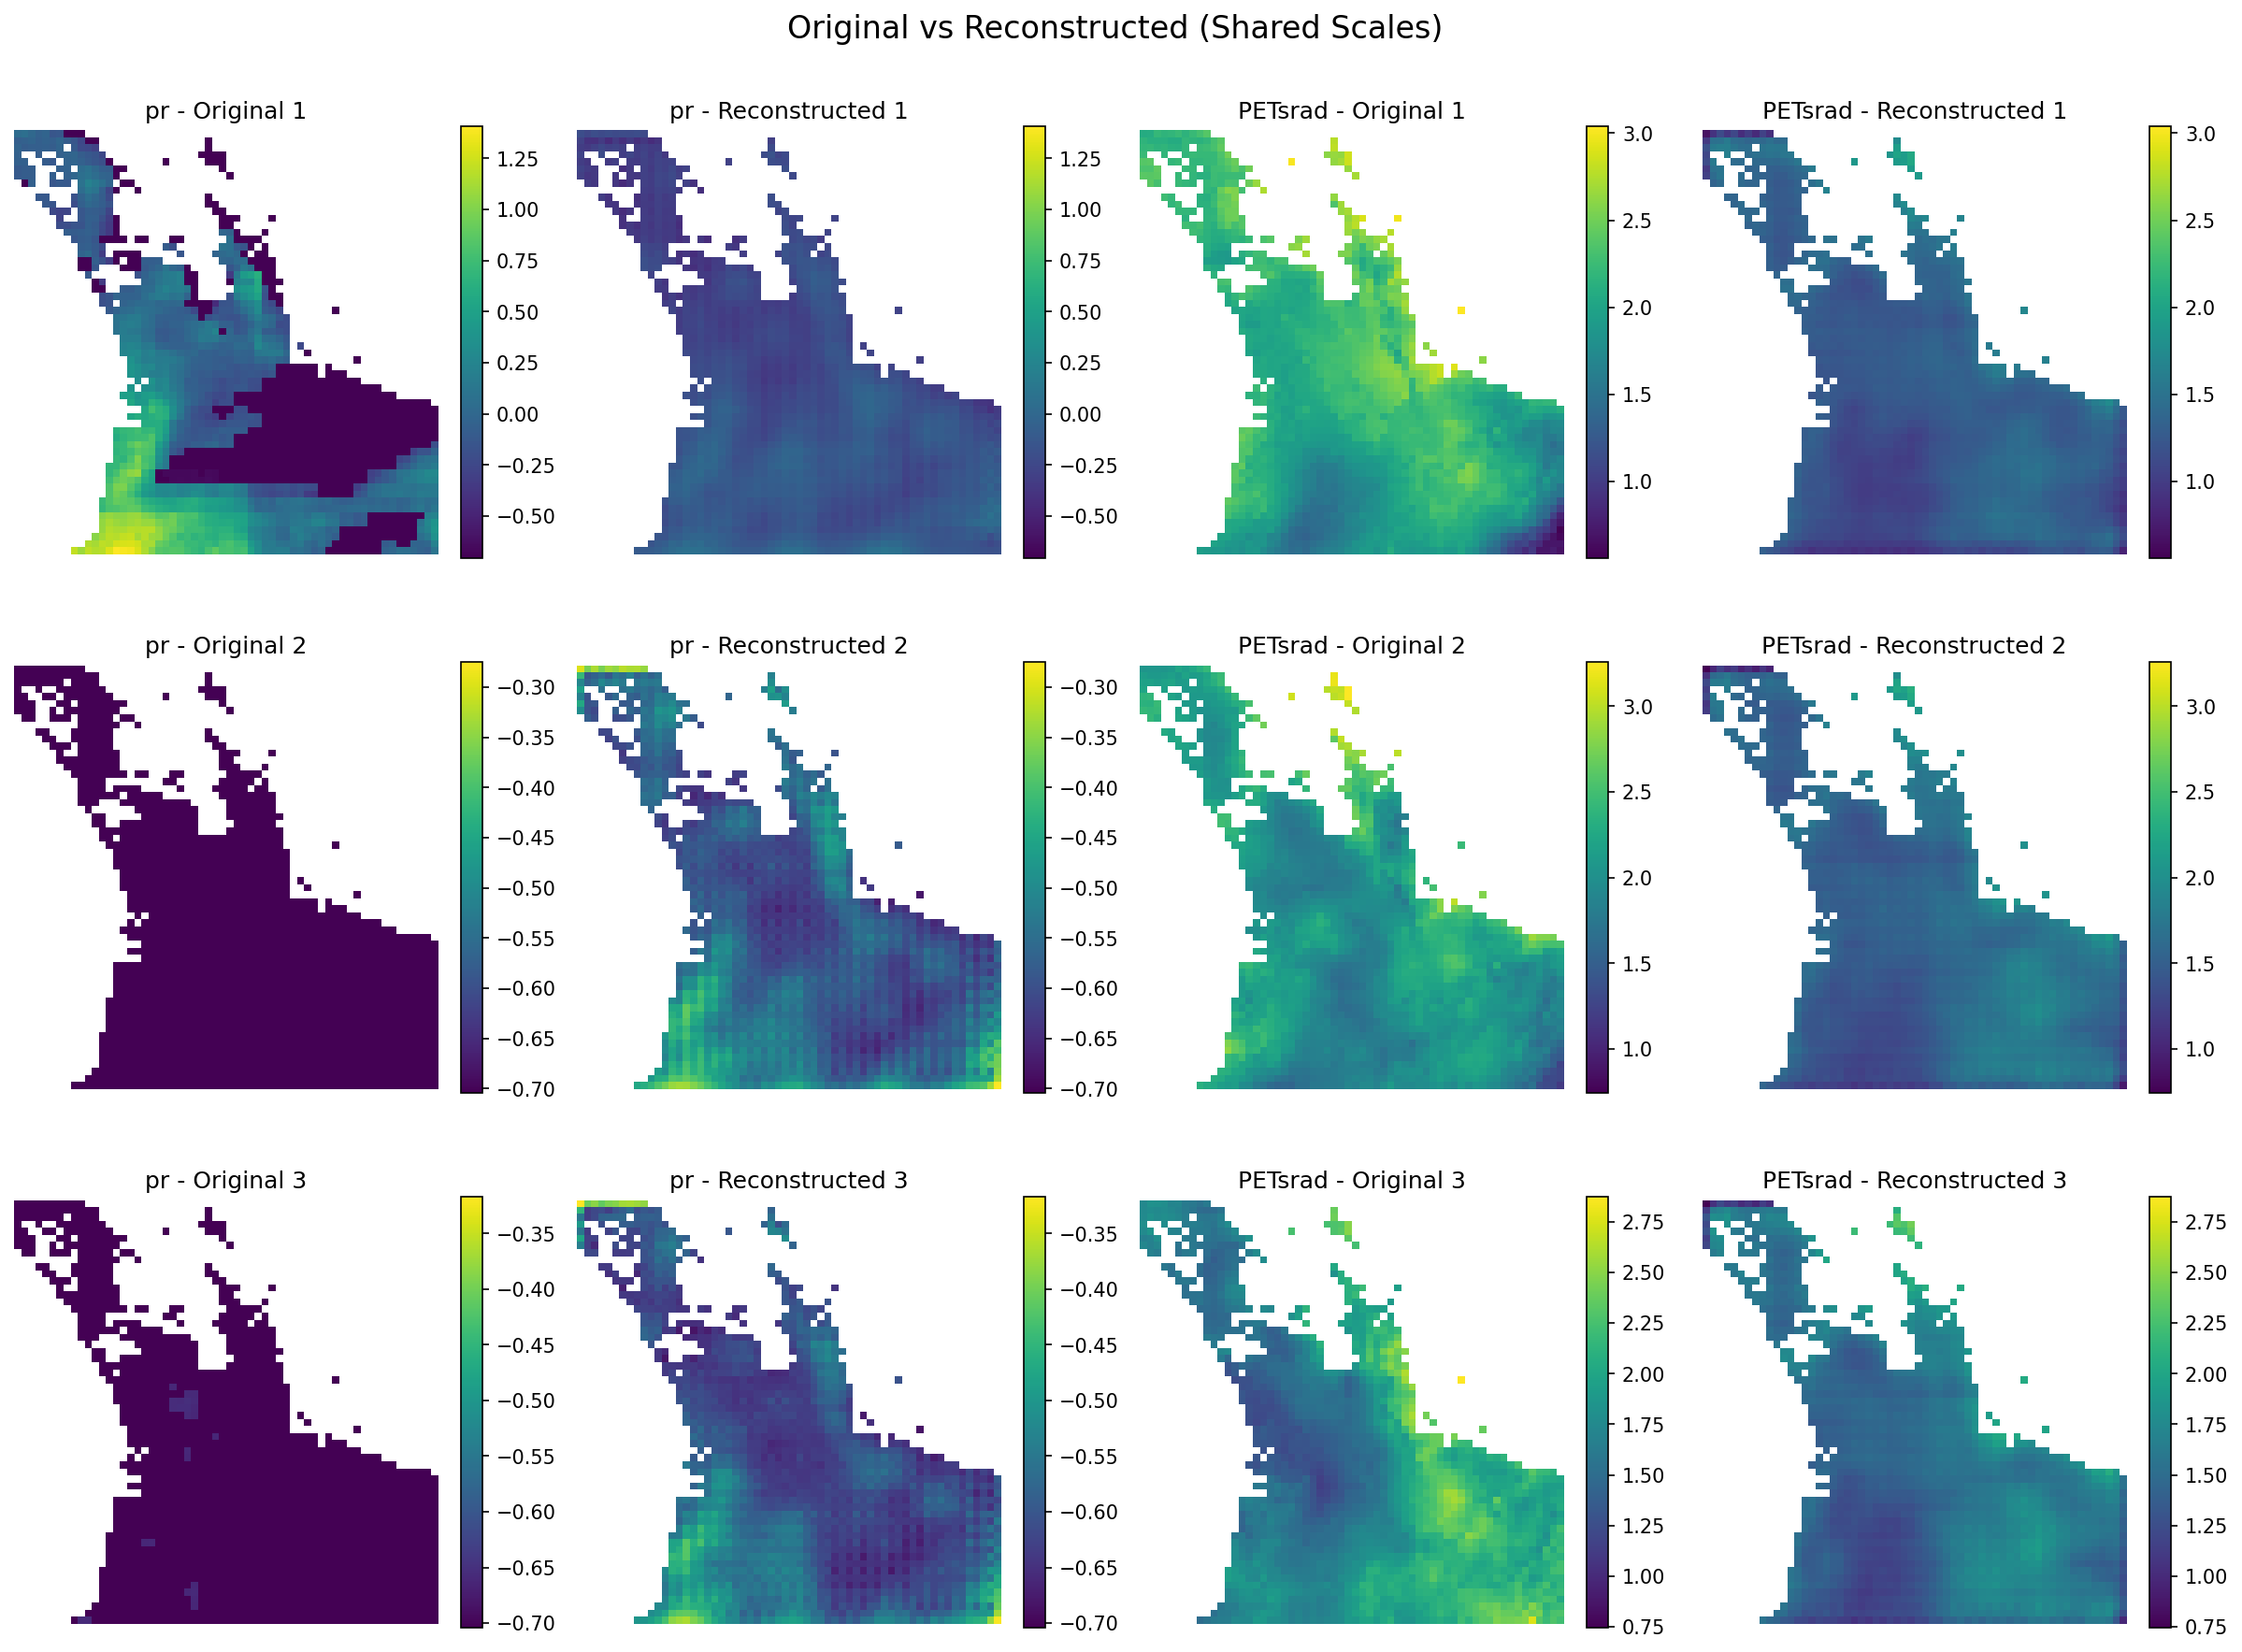
\includegraphics[scale=0.35]{figures/reconstruction_comparison.png}
    \caption{VAE Reconstructions of Randomly Sampled Events}
    \label{fig:reconstructions}
\end{figure}

\chapter{Discussion}

\chapter{Conclusion}



\clearpage
\addcontentsline{toc}{chapter}{References}
\bibliographystyle{unsrt}
\bibliography{references}

\newpage
\chapter{Appendix A} \label{AppA}


\end{document}
